
\chapter{Software and technology}

\pagestyle{fancy}

The clasic concept of a GIS is that of a complete software application which implements all the tools needed for working with geographical data: creating or editing it, managing it, analysing it and visualizing it. Along with that, other types of applications have appeared which, although they do not match exactly that definition, have to be considered as part of the GIS world as well.
We will divide GIS applications in three main blocks: desktop GIS, web-based GIS, and mobile GIS. They will be described in detail in this chapter. We will also provide additional information about some technologies that they are based one.


\section{Desktop GIS}

Five are the fundamental functionalities of a desktop GIS: \textbf{data input and output, visualization, editing, analysis, and map creation}. Most desktop GIS tools have these five capabilities, although the level of functionality for each of them might differ. Some tools might be more prepared for data editing, while others might focus mainly on analysis.

\subsection{Data input and output}

A desktop GIS must be able to \textbf{read data} and, optionally, to \textbbf{save} it. This last functionality is needed in case the GIS can produce new layers, but not in those ones that do not contain analysis or editing capabilities.

There is a very large number of data formats for \textbf{geographical data}, and most GIS use common libraries to be able to read and write them, which allows them to share data between them and improve their connectivity.

Apart from being able to read data files, nowadays it is also important to be able to connect to \emph{databases} and \textbf{remote services}. We will talk about them later in this same chapter.

\subsection{Visualization}

Visualization is a fundamental capabilities of GIS. It is, of course, important when the main purpose of using a GIS is to create cartography, but also when our work is focused on data editing or analysis, since visual exploration of the data is a previous step.

The visualization part of a GIS is mainly comprised of \textbf{canvas} on which layers are rendered. The user can add or remove layers, and also change their \textbf{symbology}, that is, the way in which the layer data is converted into graphical elements. Layers are rendered in a given order, which allows to create a \emph{rendering hierarchy}.

Along with the canvas, there are \textbf{navigation tools} that allow the user to modify the area that is being displayed, by zooming in, zooming out or panning (Figure \ref{Fig:Navigation_tools}). 

\begin{figure}[!hbt]
\centering
\includegraphics[width=.99\textwidth]{Software/Navigation_tools.png}

\caption{\small Navigation tools that are common in a desktop GIS. a) zoom out, b) zoom in, and c) pan}
\label{Fig:Navigation_tools} 
\end{figure}

The most remarkable feature of geographical data visualization in a GIS is that, unlike what happens with a classic printed map, where its characteristics cannot be changed, here the user can select \emph{what} he sees} and \emph{he} sees it. Geogrpahical data is \textbf{independent of the information needed to visualize it}, and, therefore, it can be represented in different ways. This is true even for data that has an inherent visual nature, such as images, since even in that case the rendering can be adjusted and modified by the user.

Although in the most common case the canvas is bidimensional, certain GIS are also capable of \textb{three-dimensional rendering}. In this case, navigation tools are more complex, and they allow to adjust perspective, vision angles or vertical exaggeration, among other parameters.

\subsection{Analysis}

Analysis is a fundamental functionality of GIS since its origins. Other ones, such as visualization, although we cannot imagine GIS without them nowadays, were vey limited in the early days. Analysis, however, has always been at the core of GIS.

The current trend in GIS is to consider analysis capabilites as \textbf{modular tools} that are run on a base platform, which includes the data input and output capabilities, along with the visualization component. Analysis tools are independent, but they can be used together to create more complex analyses.

Analysis tools might be completely independent of the visualization part, or be linked to it. In the first case, the analysis is performed on a set of layers and parameters without any interaction with the <<map>>, while in the second case the user might interact with the view to define how the analysis is performed (for instance, selecting a coordinate or a region in the canvas, which will then be used as a parameter for the analysis tool).

The result of an analysis tool in a GIS can be geograhical (a new layer) or not (a simple value, such as the one resulting from some statistical analysis of the input data).

Analysis tools can be organized into \textbf{workflows} which help\textbf{automate} analysis routines. Also, the analysis functionality of desktop GIS can usually be used from \emph{scripting languages}, which allow to define more complex models and data flows. this is one of the main strengths of current GIS tools, since it provides the user more power and flexibility.

\subsection{Editing}

The geographical data with which we work in a GIS are not static. Information contained in a layer \textbf{might have to be changed or corrected}, and the functionality that allows the user to do that is important if we want the GIS tool to be versatile. Without them, geographical data lose part of their potential, and that's the reason why most desktop GIS tools implement editing capabilities to some extent.

This capabilities can be used to \textbf{create new layers} or to \textbf{update existing ones}. The following are some editing tasks that can be performed with a GIS:

\begin{itemize}
\item Editing the geometries of a vector layer feature.
\item Editing the attribute values of a vector layer feature. That includes editing the list of attributes of the layer, adding or removing them.
\item Adding new features to a vector layer or removing existing ones.
\item Editing cell values in a raster layer.
\end{itemize}

Tools used to edit geometries inherit a large part of their design from CAD sofware. In certain case, they are extendend with new functionalities, as it happens in the case of editing geographical data with topology (CAD software does not consider topology).


\subsection{Map creation}

Most desktop GIS are capable of producing cartographic documents which can later be printed and used as a classic paper map. These documents are composed in the GIS from the its data, and use the same functionality that it has for the on-screen rendering (symbology, etc)

Along with that, other tools allow to \textbf{design and compose the map}, and to \emph{adjust its elements} (rendered layers, legend, title, etc.), and are inspired by those found in design software. 

Some desktop GIS include elements to \emph{automate cartographic production}, such as templates or tools to generate map series (Figura \ref{Fig:Map_series}).

\begin{figure}[!hbt]
\centering
\includegraphics[width=\textwidth]{Software/Map_series.png}
\caption{\small Automated creation of map series in a GIS.}
\label{Fig:Map_series} 
\end{figure}

This is possible thanks to the \textbf{separation between geographical data and the design of the cartographic document}, similar to what we commented for the case of visualization.


\section{Web mapping. Clients and servers}

One of the most relevant advances in the history of GIS is the advent of \textbf{Web mapping}. Web mapping technologies are used to incorporate GIS elements as part of websites, with internet browsers being then the base platform on which GIS functionality is executed. These technologies include not just the elements run on the browser, and they have been key in shaping hape and develop other ones such as \textbf{remote data services}, which are used by Web Mapping applications, but also by desktop GIS.

The concepts of \emph{server} and \emph{client} are fundamental in this context. Let's discuss them with a bit more of detail.

A \textbf{} is the element that provides (serves) a given content through the network. In our GIS context, this content means basically geographical data. The \textbf{client} is the element that requests the data, receives it and works with it. 

A web browser is a client, since it makes a request to get the content of a web site and show it to the user. When we enter a web address in the address bar of a web browser, we provide the information needed to establish the connection between the server and the client, and to transfer the data from one to the other.

Let's see how that works. Suppose that we want to visit the following website:

\begin{center}
\small\texttt{http://victorolaya.com/writing}
\end{center}

The requests is done based on the web address ---more technically, a Uniform Resource Locator (URL)---, which is a reference to a web resource that specifies its location on a computer network and a mechanism for retrieving it. We can divide it in the following parts:

\begin{itemize}
	\item \texttt{http}: The protocol to use, which defines the way client and serer will communicate with each other.
	\item \texttt{victorolaya.com}: The host name. This part identifies the server machine connected to the network where the page that we want to visit is stored. It is a human-readable version of a numeric code that indicates the address.
	\item \texttt{writing}: The page we want among all the ones that the server can provide. 
\end{itemize}

The process that allows us to have that page in our web browser comprises the following steps:

\begin{enumerate}
	\item The client makes the request.
	\item The server machine is identified and the request is driven to it.
	\item The server prepares the page that has been requested and sends it back to the client (or it send an error message in case it could not find or prepare the page).
	\item The client receives the page and renders it so the client can see it.
\end{enumerate}


Figure \ref{Fig:How_internet_works} shows a summary of this.

\begin{figure}[!hbt]   
\centering
\includegraphics[width=\columnwidth]{Software/How_internet_works.pdf}
\caption{\small Client-server interaction mechanism that takes place when visiting a website.}
\label{Fig:How_internet_works} 
\end{figure}

A relation is established between clients and servers, in which an arbitrary number of clients <<connect>> themselves to a server, from which they obtain data whenever each of them makes a request. In this client-server architecture, the server has the data to be shared through a service, while clients only provide information about themselves needed to validate and perform the data sharing.

Now let's see how this ideas apply to the field of GIS.

Regarding servers, they can have four main capabilities:

\begin{itemize}
\item \textbf{Serve rendered geographical data}. Generally known as \textbf{map servers}, they provide <<maps>>, that is images created from geographical data. If data is already an image (such as an aerial or satellite photograph), the server will just send it as it is. If data is not an image (vector layer or raster layer other than image), the server will create an image based on the geogrpahical data. The symbology used to do this can be a default one that the server uses for all requests, or it can be provided by the client in the request. 

In both cases, the client also specifies the dimensions of the requested map image that is served, and the server takes care of preparing it.


\item \textbf{Serve the data directly}. A more flexible option is to serve the geogrpahical data itself. The client requests the data and, once it has been transmited across the network, can use it however he needs. In case the data is to be visualized, the symbology has to be set in the client side, since the server is not taking care of that and provides the raw data.


\item \textbf{Serve the result of queries}. Another functionality that the server can have is to return not just the full set of geographical data, but a subset of it. The client can specify a \textbf{filter} and the server will use it to create a subset that will later be send in the reponse. Also, the server can provide \textbf{descriptive values} about the data it has. The client, which might be connected to several services and consume that from then, can use those values to filter which services to use (for instance, asking them the extent of their data and then selecting only those ones that have data about a given study area). As we have already seen, \textbf{metadata} have a great relevance in this context, since they allow this kind of queries to be executed (and the corresponding requests to be responded) efficiently.

\item \textbf{Serve processes}. Finally, a server can provide new data, whether geographical or not, computed from the geographical data. In this case, the server provides a processing service, as it processes the data that is passed to it as part of the request. The request can contain the data itself, or a reference to it. If a reference is passed, the data might already be in the server, or it can be in another one. In this last case, the first server will become a client of the second one, it will retrieve its data, process it, and send back the result to the original client (Figure \ref{Fig:Remote_data_and_services}).


\begin{figure}[!hbt]   
\centering
\includegraphics[width=0.95\textwidth]{Software/Remote_data_and_services.png}
\caption{\small Remote processign service using data from a second server..}
\label{Fig:Remote_data_and_services} 
\end{figure}

\end{itemize}

About clients, they can be divided in two classes:

\begin{itemize}

	\item \textbf{Heavy clients}. Heavy clients are independent applications that do not run on top of another one such as a web browser. They usually have a larger size, since the application has to care of all the program logic.

	Heavy clients handle and use data not coming from web services, such as local data files. They are not just clients, but full-fleged applications that work even without its client part.

	Nowadays, most desktop GIS are heavy clients themselves, since they have the functionalty of classic GIS, but can also consume web services.


	\item \textbf{Light clients}. They normally have a smaller size and their capabilities are more limited. They run on web browsers and most of the tiem rely on remote data from servers.

	Although originally they focused on data visualization (adding map views to websites, with a certain degree of interactivity), they have started implementing more advances functionalities such as analysis functionality (whether on the client side or using a processing service) or data editing.

	Hablamos de clientes ligeros cuando nos referimos a \emph{Web Mapping} y a clientes que se ejecutan sobre un navegador Web, ya que estos suelen ser sencillos en cuanto a sus funcionalidades.
	
	The term \emph{Web mapping} is used to refer to the lighter clients which focus only on rendering maps, while the term \emph{Web GIS} is used to those with more functionality, which incorporate some of the tools traditionally found in desktop GIS.
\end{itemize}

\section{Some techniques related to GIS services}

Two important techniques used in the context of the client--server architecture for geographical data are \textf{tiling} and \textbf{caching}. These techniques, whether implemented on a light client or a heavy one, allow to have more responsive interfaces and to reduce the amount of data sent over the network, overcoming to a certain extent the problems that a slow network might cause. Both are used mainly with map servers (server that provide rendered images).

Tiling divides the images that the client is working with into smaller ones, forming a mosaic. By correctly managing the tiles in that mosaic, the amount of data transmitted can be reduced. When the request is sent to the server, instead of a single image, a set of them is requested. Although this does not reduce the amount of data, the tiled structure will allow a more flexible and optimized handling of data once a new image is needed, as it will soon be explained.

Caching is technique frequently used not just for web SIG, but as a general tool in the context of the Internet context. Web browsers store previous responses from web servers, such as web pages and images, in a so-called \emph{cache}. When data that was previously requested is requested again, it can be taken from the cache instead of from the corresponding server, which is usually faster and more efficient.

Combining tiling and caching increasing responsiveness and results in an optimized data management. Let's see how that works, using the example shown in figure \ref{Fig:Tiling} 

\begin{figure}[!hbt]   
\centering
\includegraphics[width=\textwidth]{Software/Tiling.pdf}
\caption{\small Combination of tiling and caching techniques to optimize data handling in a web GIS application.}
\label{Fig:Tiling} 
\end{figure}

Initially, the application displays an area that cover 20 elements or tiles. All those tiles have already been downloaded from the server, and stored in the application cache, which means that using them again does not require making a new request to the server. Without caching and tiling, when the application user changes the area to be displayed as shown in the figure, a whole image has to be requested, exactly with the same size as the image to be rendered in the screen. However, if tiling and caching are applied, we just have the whole new image to be painted divided in 20 parts, and, since some of them are stored from a previous request, we just have to request a small number of them (8 in this case, corresponding to the areas not covered by the previous image). The amount of data that is requested to the server and transmitted over the network is much smaller.

Caching can also be implemented on the server side. We have seen that map servers provide already rendered images based on some data. Rendering that data can be time consuming, and if it has to be done for each requests, that would mean a lot of computing cost for the server. Instead, images are pre-rendered at different scales, so when a client request is received by the server, it just has to crop the pre-rendered image instead of producing the response image from the base data.

A recent technique that is gaining popularity is \emph{vector tiling}. Using the same approach as in the case of the tiling we have just seen (that is, cutting the data and in pieces), vector layers are divided and only the required data are sent to the client.

This allows the client to request and use vector layers, and be responsive at the same time. Without vector tiling, this would be impossible for large layers. The advantage of vector data in this case is that the symbology can be defined by the client. Also, the user experience is improved, since, for instance, transitions become more fluent when changing the map scale, due to the scalability of vector data.




\section{Standards}

To ensure the the client-server system works correctly, it is important to define how the communication between servers and clients takes places. Some \textbf{normalization} is needed, and there must be common and well-defined elements implemented by both the client and the server. This \emph{lingua franca} that allows clients and servers to communicate is what we call a \textbf{standard}.

In an ideal situation, a complete \textbf{interoperability} would exist, indepentently of formats and applications used. Clients and servers would be able to connect with each other, regardless of their own characteristics. Standards are the element that allows that to happen, since they define a common framework in which clients and servers will communicate. As long as a client or a server follows the standard, it will be able to communicate with all others that do it as well. Standards provide \textbf{technological homogeneity}.


Interoperability means that any element of the client-server system can be replaced with another one, and the interaction between all parts of the system will not  be affected. A client or server might gave different functionalities, but regardless of its origin (its manufacturer), it will be able to interact with the other elements, if all implement the same standard.

A standard is considered as such when it is used by a group or community, which accepts it to define the characteristics of a product or service within it. Standards can be established by public acceptance and custom (\emph{de facto} standards), or they might have legal recognition and be proposed by some oficial organization (\emph{de iure} standards).

A standard is \textbf{open} if \textbf{its definition is available} to everyone who wants to know more about it and use it for any activity related to it.

The following ones are some of the fundamental principles that open standards are based on:

\begin{itemize}
	\item \textbf{Availability}. Open standards are available to anyone, to read and to use.
	\item \textbf{Maximize end-user choice}. Open standards create a fair, competitive market, and do not lock users in the closed environment of a given vendor. 
	\item \textbf{No royalty}. Implementing a standard is free and has no cost, unlike the case of a patent.
	\item \textbf{No discrimination}. Open standards and the organizations behind them do not favor any implementor of the standard over the rest of them.
	\item \textbf{Extension or creation of subsets}. Standards can be extended with additional elements, or reduced to less-detailed subsets.
\end{itemize}

To know the impact that a standard has in the context of GIS, let's take a look at figure \ref{Fig:Non_interoperable}, which represents a non-interoperable architecture that does not use standards.

\begin{figure}[!hbt]   
\centering
\includegraphics[width=.7\columnwidth]{Software/Non_interoperable.pdf}
\caption{\small Non-interoperable architecture.}
\label{Fig:Non_interoperable} 
\end{figure}

Data stored in each data base are available only by using one client, the one corresponding the the server that serves those data. The remaining data are not available for that client. Each client-server-database group is an independent island, technologically isolated from the rest of them.

Among the disadvantages of a non-interoperable architecture like that, we find the following ones:

\begin{itemize}
\item \textbf{Waste of resources}. Each service must manage its own data. That is complex and has higher costs than sharing data with other compatible services.
\item \textbf{Need to know multiple clients}. Since we need a different client for each service, the user must be familiar with all of them. Being capable of using just one client is not enough to use all the available data, since that client can only access a small part of all that data..
\item \textbf{Combining data is not possible}. Two datasets that are available through two different services cannot be used in the same client, since it cannot communicate with the corresponding servers.
\item \textbf{Combining functionalities is not possible}. If data is only available to a given client, the functionality in another one (which might not be implemented in the first) cannot be used on that data. When working with that data, the user has its possibilities limited to what the corresponding client can do.
\end{itemize}

Now let's take a look at a fully interoperable architecture based on open standards, as seen in figure \ref{Fig:Interoperable}.

\begin{figure}[!hbt]   
\centering
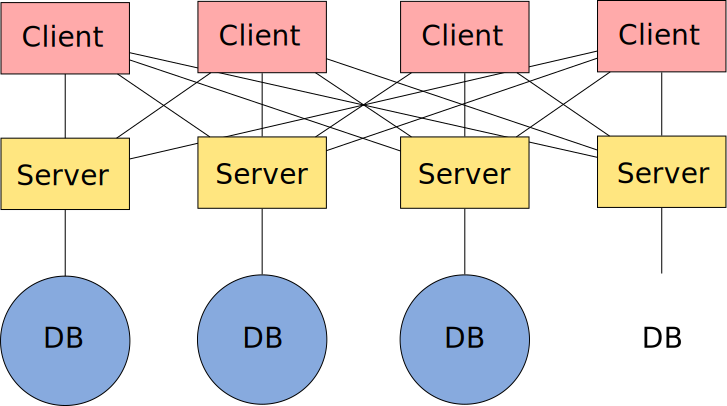
\includegraphics[width=.7\columnwidth]{Software/Interoperable.pdf}
\caption{\small Interoperable architecture.}
\label{Fig:Interoperable} 
\end{figure}

In this case, there is a server that manages and offers the services for each database, but all clients can access all servers, since they are based on open standards and communication is possible between any two of them.

\subsection{Relevant standards in GIS}

The most common standards for geographical information are created and promoted by the  \textbf{Open Geospatial Consortium (OGC)}. The OGC is <<an international not for profit organization committed to making quality open standards for the global geospatial community>>.

Some of the most relevant OGC standards are the following ones:

\begin{itemize}
\item \textbf{WMS}. To serve maps (images)
\item \textbf{WCS}. To serve coverages (currently only raster layers).
\item \textbf{WFS}. To serve geographical features and attributes (vector layers). It can also allow editing features from the client.
\item \textbf{WPS}. To serve remote processing services.
\item \textbf{GML}. To store geographical information.
\item \textbf{CSW}. To make queries to a catalog that contains geographical data.
\end{itemize}

Each one of these standards is describen in the corresponding specification, which is subject to change and improvement. Several versions exist for each of them.

Along with these standards, we find those made by organizations such as \textbf{ISO} o \textbf{W3C}, with a more general scope, but also important in the context of GIS. Among them, the most relevant standards are the ISO ones that define \textbf{how to store metadata} and the W3C ones related to \emph{communication over the Internet}.

\section{Mobile GIS}

GIS on mobile platforms such as mobile phones or tablets has a clear relation with both desktop GIS and web GIS. It takes the elements from them and adds  additional ones derived from the running on a mobile platform, which expand its posibilities.

Mobile devices nowadays offer two main capabilities from the point of view of GIS: \textbf{wireless access to Internet} and \textbf{capability of knowing the position} of the device. 

Intenet access can be used to obtain maps and geographical information from a given server, or to send field data acquired with the aid the mobile device.

The position of the mobile device is usually known based on the GPS receiver that is part of most mobile phones. However, other approaches are also possible, from computing the position \textbf{based on the phone network} to using some \textbf{indoor positioning system} in case it is available.

Knowing the position of the device allows the mobile GIS application to provide additional functionality. For instance, it might be used to make \textbf{field data aquisition} easier and more efficient(the coordinates of measured points do not have to be entered manually), or to provide \textbf{location-based services} (LBS).  

Some of the main groups in which these services can be grouped are listed next.

\begin{itemize}
	\item \textbf{Navigation}. Shortest path computation, route guidance, etc.
\item \textbf{Data acquisition}. Any type of data can be registered in the field, and the device associates to them its own position automatically.
\item \textbf{Information}. Business directories, travel guides, etc.
\item \textbf{Advertising}. Location-based advertisements, promotions for nearby shops, etc.
\item \textbf{Tracking}. Of both people and products, along predefined routes or arbitrary ones.
\item \textbf{Management}. Of infrastructures, installations or fleets.
\end{itemize}

When running in a mobile platform, a GIS has additional information about the context it is running on (position, direction of movement, speed, illumination, etc.), that it can use to provide more functionality than a desktop or web GIS running on a non-mobile platform.

\pagestyle{empty}
